% Options for packages loaded elsewhere
\PassOptionsToPackage{unicode}{hyperref}
\PassOptionsToPackage{hyphens}{url}
%
\documentclass[
  11pt,
  a4paper,
]{article}
\usepackage{amsmath,amssymb}
\usepackage{lmodern}
\usepackage{iftex}
\ifPDFTeX
  \usepackage[T1]{fontenc}
  \usepackage[utf8]{inputenc}
  \usepackage{textcomp} % provide euro and other symbols
\else % if luatex or xetex
  \ifXeTeX
    \usepackage{zxjatype} 
    \usepackage[ipaex]{zxjafont}
    \setromanfont{Times New Roman}
  \fi
  \usepackage{unicode-math}
  \defaultfontfeatures{Scale=MatchLowercase}
  \defaultfontfeatures[\rmfamily]{Ligatures=TeX,Scale=1}
\fi
% Use upquote if available, for straight quotes in verbatim environments
\IfFileExists{upquote.sty}{\usepackage{upquote}}{}
\IfFileExists{microtype.sty}{% use microtype if available
  \usepackage[]{microtype}
  \UseMicrotypeSet[protrusion]{basicmath} % disable protrusion for tt fonts
}{}
\usepackage{xcolor}
\IfFileExists{xurl.sty}{\usepackage{xurl}}{} % add URL line breaks if available
\IfFileExists{bookmark.sty}{\usepackage{bookmark}}{\usepackage{hyperref}}
\hypersetup{
  pdftitle={Text-Based Nudges Promoting Rubella Antibody Testing and Vaccination: Evidence from Nationwide Online Field Experiment in Japan},
  hidelinks,
  pdfcreator={LaTeX via pandoc}}
\urlstyle{same} % disable monospaced font for URLs
\usepackage[left=3cm,right=3cm,top=3cm,bottom=3cm]{geometry}

\usepackage{setspace}
\renewcommand{\baselinestretch}{2}
\usepackage{float}

\usepackage{longtable,booktabs,array}
\usepackage{threeparttable, threeparttablex, multirow}
\usepackage{calc} % for calculating minipage widths
% Correct order of tables after \paragraph or \subparagraph
\usepackage{etoolbox}
\makeatletter
\patchcmd\longtable{\par}{\if@noskipsec\mbox{}\fi\par}{}{}
\makeatother
% Allow footnotes in longtable head/foot
\IfFileExists{footnotehyper.sty}{\usepackage{footnotehyper}}{\usepackage{footnote}}
\makesavenoteenv{longtable}
\usepackage{graphicx}
\makeatletter
\def\maxwidth{\ifdim\Gin@nat@width>\linewidth\linewidth\else\Gin@nat@width\fi}
\def\maxheight{\ifdim\Gin@nat@height>\textheight\textheight\else\Gin@nat@height\fi}
\makeatother
% Scale images if necessary, so that they will not overflow the page
% margins by default, and it is still possible to overwrite the defaults
% using explicit options in \includegraphics[width, height, ...]{}
\setkeys{Gin}{width=\maxwidth,height=\maxheight,keepaspectratio}
% Set default figure placement to htbp
\makeatletter
\def\fps@figure{htbp}
\makeatother
\setlength{\emergencystretch}{3em} % prevent overfull lines
\providecommand{\tightlist}{%
  \setlength{\itemsep}{0pt}\setlength{\parskip}{0pt}}
\setcounter{secnumdepth}{5}
\newlength{\cslhangindent}
\setlength{\cslhangindent}{1.5em}
\newlength{\csllabelwidth}
\setlength{\csllabelwidth}{3em}
\newlength{\cslentryspacingunit} % times entry-spacing
\setlength{\cslentryspacingunit}{\parskip}
\newenvironment{CSLReferences}[2] % #1 hanging-ident, #2 entry spacing
 {% don't indent paragraphs
  \setlength{\parindent}{0pt}
  % turn on hanging indent if param 1 is 1
  \ifodd #1
  \let\oldpar\par
  \def\par{\hangindent=\cslhangindent\oldpar}
  \fi
  % set entry spacing
  \setlength{\parskip}{#2\cslentryspacingunit}
 }%
 {}
\usepackage{calc}
\newcommand{\CSLBlock}[1]{#1\hfill\break}
\newcommand{\CSLLeftMargin}[1]{\parbox[t]{\csllabelwidth}{#1}}
\newcommand{\CSLRightInline}[1]{\parbox[t]{\linewidth - \csllabelwidth}{#1}\break}
\newcommand{\CSLIndent}[1]{\hspace{\cslhangindent}#1}


\usepackage{float}
\usepackage{threeparttable}
\ifLuaTeX
  \usepackage{selnolig}  % disable illegal ligatures
\fi

\title{Text-Based Nudges Promoting Rubella Antibody Testing and Vaccination:
Evidence from Nationwide Online Field Experiment in Japan  \thanks{This study is conducted as a part of the Project ``Implementation of EBPM in Japan''
undertaken at the Research Institute of Economy, Trade and Industry (RIETI).
In completing this paper,
we thank participants of the EBPM Study Group and
the Discussion Paper Study Group of RIETI for their insightful comments.
This research is financially supported by
the Japan Society for the Promotion of Science
{[}JSPS Grant Number: 20H05632 (F., Ohtake){]}
and the Ministry of Health, Labor, and Welfare.
Prior to conducting a randomized controlled trial on an online survey,
this study was approved by the Institutional Review Board
of the Graduate School of Economics, Osaka University (R020114).}  }
\author{
    Hiroki Kato
  \thanks{Graduate School of Economics, Osaka University. E-mail: h-kato@econ.osaka-u.ac.jp  }
  \and
    Shusaku Sasaki
  \thanks{Center for Infectious Disease Education and Research, Osaka University.  }
  \and
    Fumio Ohtake
  \thanks{Graduate School of Economics, Osaka University.
Center for Infectious Disease Education and Research, Osaka University.  }
  \and
  }

\date{2022/05/30}



\begin{document}
\begin{spacing}{1}
  \maketitle
\end{spacing}
\begin{spacing}{1}
  \begin{abstract}
    This study conducted a randomized controlled trial (RCT) in a nationwide online survey
    to examine which text-based nudges best promote rubella antibody testing and vaccination.
    The main results are as follows.
    First, the altruistic message,
    which emphasizes that the fetus's health could be impaired by
    infecting women in the early stages of pregnancy with rubella,
    has a positive effect on the intention and behavior relating to the antibody test among men,
    who had automatically received a free coupon from the local government in 2019.
    Second, most people who test negative for antibodies (do not have antibodies),
    regardless of the type of nudge messages or whether or not they have received the coupon,
    have since been vaccinated.
    This result suggests that policies to increase antibody testing of pre-test individuals
    should be prioritized over those to increase vaccination of post-test negatives.
    Third, text-based messages have no statistically significant effect
    among men who had to apply for coupons themselves in 2019.
    
                \noindent
    \textbf{Key words}: Rubella, Vaccination, Antibody Test, Text-Based Nudges
        
        \noindent
    \textbf{JEL Codes}: D90, I12, I18
            
  \end{abstract}
\end{spacing}

\hypertarget{intro}{%
\section{Introduction}\label{intro}}

\hypertarget{background}{%
\section{Background of Rubella Vaccination in Japan}\label{background}}

\begin{figure}[t]
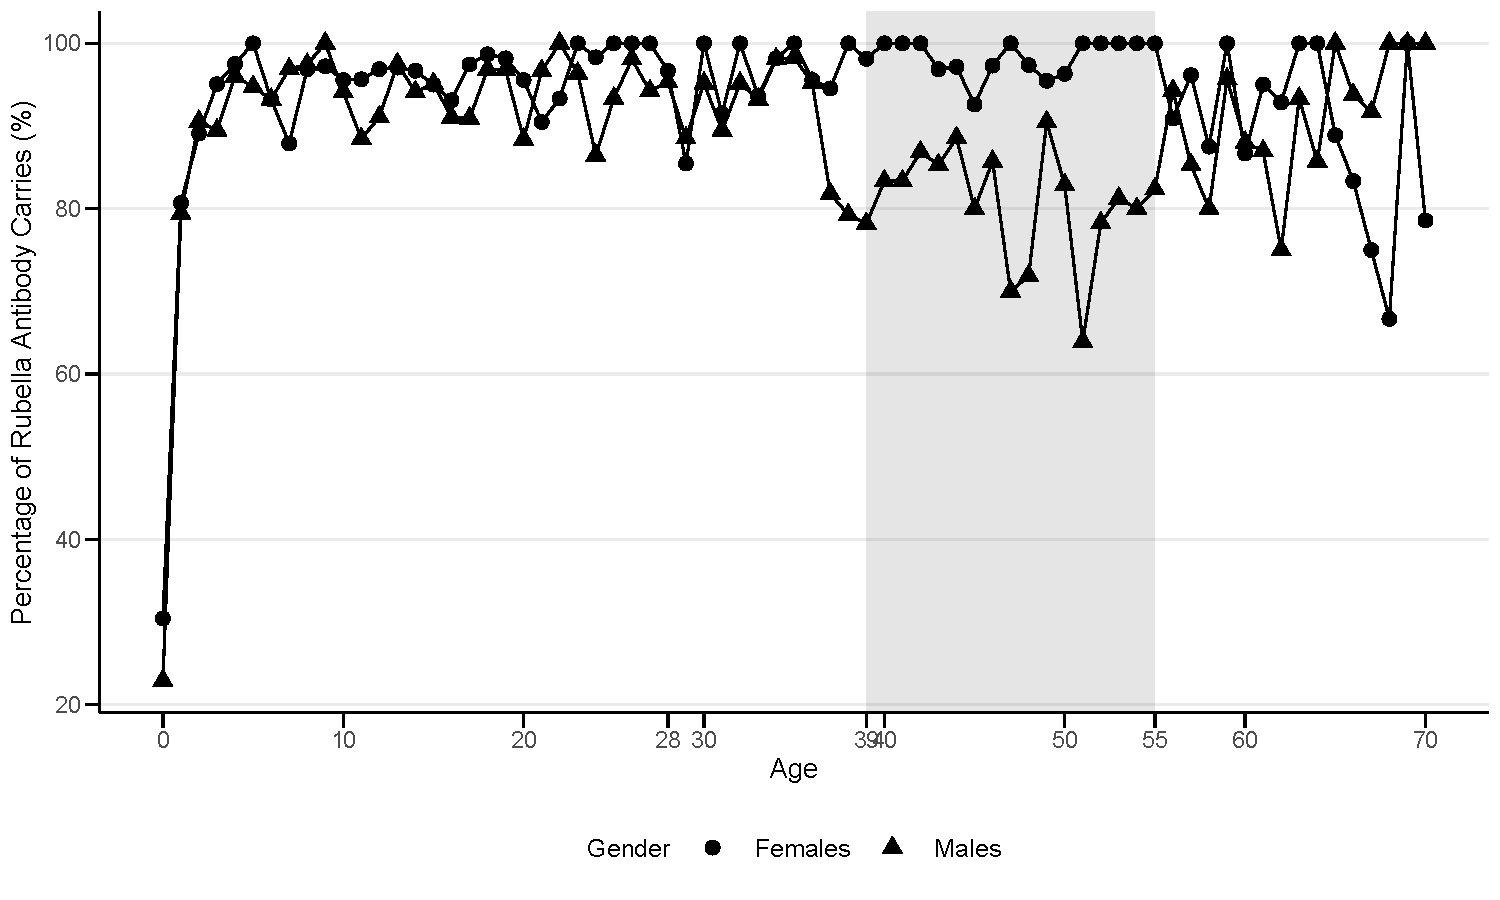
\includegraphics{C:/Users/vge00/Desktop/MHLW-Rubella-Project/2020-online-RCT/publish/body_files/figure-latex/niid-antibody-1} \caption{Percentage of Rubella Antibody Carriers at Each Age by Gender. Data: NIID "2018 National Epidemiological Surveillance of Vaccine-Preventable Diseases (NESVPD)."}\label{fig:niid-antibody}
\end{figure}

図\ref{fig:niid-antibody}は国立感染症研究所(NIID)の2018年度感染症流行予測調査を使って、
日本の男女別・年齢別の風しん抗体保有率をプロットしたものである。
39-55歳の男性の抗体保有率は約80.7\%であり、
同じ世代の女性(約98.3\%)や他の世代と比較して低いことが分かる\footnote{このデータを用いて、3つの年齢層(38歳以下・39歳以上55歳以下・56歳以上)と
  女性ダミーの飽和モデルによって抗体保有率を予測した。
  その結果、39歳以上55歳以下の抗体保有率の男女差は
  0.176 (std.error = 0.034; p = 0.000)
  である。また、39歳以上55歳以下の男性と56歳以上の男性の抗体保有率の差は
  0.106 (std.error = 0.036; p = 0.003)
  である。}。
これは他の性年代と違って、
39-55歳の男性が定期接種として風しんワクチンを接種していないこと、
さらに、彼らの内の一部が風しんに自然感染していないことを反映している\footnote{風しんワクチンの定期接種の背景は補論に詳細を記した。}。
38歳以下の男性と女性の抗体保有率はそれぞれ91.3\%と94.0\%である。
彼らは定期接種を通じて少なくとも1回の風しんワクチンを接種している。
56歳以上の男性と女性の抗体保有率はそれぞれ91.3\%と89.4\%である。
彼らは風しんワクチンの定期接種を受けていないが、
風しんが流行していた期間に育っているので、
感染を通じて抗体を保有している可能性が高い。

Kinoshita and Nishiura (2016) によれば、
すべての世代で抗体保有率が90\%を超えれば、
日本で風しんの集団免疫が獲得できる。
これを達成するために、厚生労働省は2019年4月から2022年3月までの間で、
2019年時点で40-56歳の男性を対象にして、
風しん定期接種の追加対策を実施することを決めた\footnote{より正確には、1962年4月2日から1979年4月1日生まれの男性である。}。
この追加対策は予防接種法に基づく定期接種であり、
対象となる男性は無料で抗体検査とワクチン接種を受けられる。
ワクチン接種の効率的な活用のために、対象の男性は、はじめに抗体検査を受検する。
抗体検査により抗体が持っていないことが明らかになった男性は風しんワクチンを接種する。
この追加的対策の政策目標は、2022年3月までに、
対象世代の男性の抗体保有率を80\%から90\%に引き上げることである。

追加対策を円滑に進めるために、
厚生労働省の定めるのガイドラインのもとで、
地方自治体が風しんの抗体検査とワクチン接種の無料クーポン券を
3年かけて以下のように段階的に対象世代の男性に送付した。

\begin{enumerate}
\def\labelenumi{\arabic{enumi}.}
\tightlist
\item
  2019年度は、40-46歳の男性にクーポン券が送付される。
\item
  2020年度は、47-52歳の男性にクーポン券が送付される。
\item
  2021年度は、53-56歳の男性にクーポン券が送付される。
\end{enumerate}

2019-2020年度では、
市区町村の判断もしくは本人の希望によって、
送付対象以外の男性もクーポン券を受け取れる。

本研究は、2020年1-3月にオンライン調査を実施し、2019年度終了時点の行動に焦点を当てる。
厚生労働省の集計データによると、
2020年1月時点で、クーポン券を利用した抗体検査の受検率は約18\%と低い水準にとどまった\footnote{2019年4月から2020年3月までに40歳から46歳の男性にクーポン券が発送された。
  40-46歳の男性は約646万人おり、追加対策の対象である男性の半数以上を占める。
  厚生労働省の聞き取り調査によると、
  2019年10月までに約96\%の自治体がクーポン券の発送を完了する予定であった。
  2019年1月までのクーポン券を利用した抗体検査の累積実績件数は117万件であった。
  抗体検査の受検率は2019年1月までのクーポン券を利用した抗体検査の累積実績件数(117万件)
  を2019年度のクーポン券の発送対象年齢層の40歳から46歳の男性の人口(646万人)で割った値である。
}。

\hypertarget{experiment}{%
\section{Nationwide Online Survey Experiment}\label{experiment}}

本研究は、厚生労働省とのコラボレーションの下で、
インターネット調査会社であるマイボイスコム株式会社に委託して、
全国規模のオンライン調査を2回実施した。
我々は第1回調査を、2020年2月15日-17日に、
日本全国に居住する40-59歳の男性4,200名を対象にして実施した。
彼らは追加対策の対象で、
2019年にクーポン券が自動送付された人々とされなかった人々の両方が含まれている。
第1回調査の目的は、ナッジ・メッセージをランダムに割当て、
それらの介入が風しんの予防意向にどのような影響を与えるかを検証することである。
続いて、我々は第2回調査を、2020年3月17日-25日に、
第1回調査の回答者を対象にして行い、3,963名から回答を得た(脱落率=5.64\%)。
第2回調査の目的は、第1回目調査でランダムに割り当てたナッジ・メッセージが
実際の予防行動にどのような影響を与えるかを検証することである。

調査の詳細は補論Bに示した。
また、我々はオンライン調査上のランダム化比較試験を実施するときに、
大阪大学経済学研究科の倫理委員会の承認を事前に取得している(承認番号:R020114)。

\hypertarget{wave1}{%
\subsection{Wave 1: Treatments and Outcome Variables on Intention}\label{wave1}}

\begin{table}

\caption{\label{tab:nudgelist}List of Text-Based Nudges}
\centering
\fontsize{9}{11}\selectfont
\begin{tabular}[t]{l>{\raggedright\arraybackslash}p{20em}cccccc}
\toprule
\multicolumn{3}{c}{ } & \multicolumn{4}{c}{Age (as of Apr 2019)} & \multicolumn{1}{c}{ } \\
\cmidrule(l{3pt}r{3pt}){4-7}
Message & Contents &   & 39 & 40-46 & 47-56 & 57-59 & All\\
\midrule
MHLW (Control) & Dear all men born in 1962-1979. Get a rubella antibody test and vaccination to protect yourself and your upcoming generation! & N & 20 & 210 & 321 & 49 & 600\\
MHLW (Age) & Dear men in their 40s and 50s (all men born in 1962-1979). Get a rubella antibody test and vaccination to protect yourself and your upcoming generation! & N & 23 & 205 & 309 & 63 & 600\\
Altruistic & Dear men in their 40s and 50s (all men born in 1962-1979). If a pregnant woman becomes infected with rubella because of you, her baby may be born with a disability. Get a rubella antibody test and vaccination! & N & 24 & 214 & 296 & 66 & 600\\
Selfish & Dear men in their 40s and 50s (all men born in 1962-1979). When an adult male is infected with rubella, it can become severe, and lead to complications such as encephalitis and thrombocytopenic purpura. Get a rubella antibody test and vaccination! & N & 16 & 225 & 302 & 57 & 600\\
Social comparison & Dear men in their 40s and 50s (all men born in 1962-1979). One in five people in your generation does not have rubella antibodies, which means that more than twice as many people can get rubella as compared to other generations. Get a rubella antibody test and vaccination! & N & 18 & 204 & 321 & 57 & 600\\
Deadline & Dear men in their 40s and 50s (all men born in 1962-1979). The coupon for free rubella antibody test and vaccine is valid on March 31, 2020. Get a rubella antibody test and vaccination! & N & 18 & 216 & 299 & 67 & 600\\
Convenient & Dear men in their 40s and 50s (all men born in 1962-1979). There is an increasing number of workplaces and local governments that you can take rubella antibody tests with your coupon in addition to your usual health examinations. Get a rubella antibody test and vaccination! & N & 19 & 213 & 307 & 61 & 600\\
\bottomrule
\end{tabular}
\end{table}

我々は、表\ref{tab:nudgelist}のコントロール・メッセージと
ナッジ・メッセージの中からいずれか一つをランダムに提供した\footnote{表\ref{tab:nudgelist}に示した年齢は調査によって得られた誕生年と誕生月を用いて、
  2019年4月時点の年齢を計算した。
  2019年4月時点で40歳から56歳の男性が厚労省の追加的対策の対象であり、
  40歳から46歳の男性は1年目にクーポン券を自動的に受け取る。
  4月生まれの人はまだ誕生日を迎えていないことを仮定している。
  また、2019年4月時点での年齢であるため、調査時点で40歳の男性の一部が39歳である。}。
厚労省メッセージ(\emph{MHLW (Control)} message)がコントロールメッセージで、
風しんの抗体検査とワクチン接種を勧奨するホームページ上で用いているものである
(\emph{business-as-usual control})。
我々はどのような要素をどのような表現で強調することが効果的なのかを探るために、
厚労省メッセージに基づいた6種類の異なるナッジ・メッセージを作成した。
近年の行動科学研究には、候補となるナッジ・メッセージを複数個用意して、
どれが効果的なのかを探索するもの(e.g. Dai et al., 2021; Milkman et al., 2021)が増えており、
本研究もその流れに属する。

ナッジ・メッセージは、厚労省メッセージを(1)簡易な年齢表現と(2)行動経済学に基づいたメッセージ内容に変更している。
年齢表現メッセージ(\emph{MHLW (Age)} message)は風しんの追加対策の正確な対象年齢に加えて、
「40代・50代の男性」という平易な表現を追加した。
これは自分が接種対象者であるかどうかが容易に理解できるようにして、メッセージ自体の注意を引くことを目的としている。
年齢表現メッセージは年齢表現を変えただけで、メッセージの内容は原文と同じである。

それ以外の5つのナッジ・メッセージは年齢表現だけでなく、
行動経済学の知見に基づいたメッセージ内容に変更した。
利他強調メッセージ(\emph{Altruistic} message)は
自身が感染することで他人(特に、妊婦)にどのような損害を与えるかを具体的に記述している。
これは負の外部性を容易に想起させ、外部性を考慮する利他的な人の行動変容を促すことを目的としている。

利己強調メッセージ(\emph{Selfish} message)・社会比較メッセージ(\emph{Social comparison} message)は
風しんの抗体を持つことの価値を高めることで行動変容を促すという目的で作成された。
利己強調メッセージは自身が感染することで自分がどのような損害を受けるかを具体的に記述し、
自身が感染することで生じる自身の損害を容易に想像できるようにした。
社会比較メッセージは抗体保有率が低いことを明記して、自身が感染しやすいことを強調している。
これは風しんの感染確率を過小に見積もることを通じてワクチン接種の価値を過小に評価することを防ぐことができる。

有効期限メッセージ(\emph{Deadline} message)・低コストメッセージ(\emph{Convenient} message)は
風しんのクーポン券制度に関する内容に変更した。
有効期限メッセージはクーポンの有効期限を強調する内容である。
2019年度に配布されるクーポン券には、2020年3月31日が有効期限であることを明記していた。
このメッセージは再度その内容を明記した。
これは行動経済学的特性の一つである現在バイアスによって
抗体検査の受験やワクチン接種の実行が先延ばしされるのを防ぐ目的で作成した。
低コストメッセージは健康診断のついでに抗体検査を受診できることを明記して、簡単に受検できることを強調する内容である。
このメッセージは抗体検査の主観的なコストを抑える目的で作成した。

サンプルサイズが均等になるように、我々は7つのメッセージを年齢層別にランダムに割り当てた\footnote{調査会社が保有する年齢情報を用いて、40-44歳・45-49歳・50-54歳・55-59歳の層別にランダムに割り当てた。
  各層は1,050名で構成されていて、我々はナッジ・メッセージを均等に割り当てた(150名)。}。
したがって、各群のサンプルサイズは600人である。

第1回調査では、ランダムに割り当てられたメッセージを閲覧した直後、
回答者は抗体検査受検とワクチン接種の意向について5段階で評価する。
抗体検査受検の意向は「今、あなたは、風しんの抗体検査を受けようとどのくらい思っていますか」という質問である。
ワクチン接種の意向は「抗体検査を受けて、あなたに抗体がないと分かった場合、
あなたは、ワクチンを接種しようとどのくらい思いますか」という質問である。
それぞれの質問に対して、
回答者は「絶対に受ける」「受ける」「どちらともいえない」「受けない」「絶対に受けない」「すでに受けた」で回答する。
我々は、それぞれの意向について、「絶対に受ける」もしくは「受ける」と回答したら1を取るダミー変数を作成し、
それらを意向に関するアウトカム変数として用いる。

\hypertarget{wave2}{%
\subsection{Wave 2: Outcome Variables on Behavior}\label{wave2}}

第2回調査は第1回調査以降の実際の抗体検査の受検行動・ワクチン接種の行動を調査した。
抗体検査の受検行動は
「前回のアンケートの回答終了時から今日までの期間に、あなたは風しんの抗体検査を受診しましたか」
という質問である。
回答者は「受診した」・「受診していない」・「前回アンケートより以前に、受診済みである」から一つ選ぶ。
我々は「受検した」と回答したならば1を取るダミー変数を作成し、
それを抗体検査の受検率に関するアウトカム変数として用いる。

ワクチン接種は
「前回のアンケートの回答終了時から今日までの期間に、あなたは風しんワクチンを接種しましたか」
という質問である。
回答者は「接種した」・
「すでに抗体検査で十分に抗体があることを確認した・すでに風しんに感染したので、接種する必要がなかった」・
「すでに抗体検査で十分に抗体がないことを確認したが、まだ接種していない」・
「抗体検査の受診もワクチンの接種もしていない」・
「前回アンケートより以前に、接種済みである」
から一つ選ぶ。
厚生労働省の追加対策でワクチンを接種するためには、対象者は必ず抗体検査を受検しなければならない。
同時に、抗体検査を受けずに、自費で風しんワクチンを接種している可能性もある。
この可能性を排除するために、
我々は抗体検査の受検行動の質問に対して「受検した」と回答し、
ワクチン接種の質問に対して「接種した」と回答すると1を取るダミー変数を作成し、
それをワクチン接種率に関するアウトカム変数として用いる。
厚生労働省の政策目標は抗体を持っていない人がワクチン接種を受けることで抗体保有率を引き上げることなので、
このアウトカム変数は政策目標に直結している。

\hypertarget{result}{%
\section{Results}\label{result}}

\hypertarget{sample}{%
\subsection{Policy Target and Analysis Sample}\label{sample}}

ナッジ・メッセージの政策対象は抗体検査やワクチン接種を受けていない男性である。
そこで、第1回調査時点で抗体検査とワクチン接種を受けていない回答者に限定して、
ナッジ・メッセージの効果を推定する。
意向に関するアウトカム変数に対する効果を推定するとき、
第1回調査で過去に抗体検査を受検した、もしくはワクチンを接種したと回答した人を
除いたデータを用いる(以降、wave 1 target dataと呼ぶ)。
また、行動に関するアウトカム変数に対する効果を推定するとき、
上述の基準に加えて、
第2回調査で第1回調査以前に抗体検査を受検したもしくはワクチンを接種したと回答した人を
除いたデータを用いる(以降、wave 2 target dataと呼ぶ)\footnote{第1回調査以降に自身の接種歴を調べ直すなどによって、
  第1回調査と第2回調査の回答に違いが生じる可能性がある。
  そのため、どちらかの調査で第1回調査以前に抗体検査を受検したもしくはワクチンを接種したと回答した人を除いた。}。

さらに、我々の目的は、金銭的インセンティブを取得した状況と
追加的な取引費用を支払わないとインセンティブが取得できない状況のそれぞれで、
ナッジ・メッセージの効果を推定することである。
そのために、上記の基準で構築したデータを
2019年度にクーポン券が自動的に送付されるかどうかで分割して、
それぞれのサブサンプルにおけるナッジ・メッセージの効果を推定する。
我々は2019年度にクーポン券が自動的に送付されるかどうかを2019年4月時点の年齢で識別した。
各市区町村は2019年度に40歳以上46歳以下の男性のクーポン券を送付し、
2020年度以降に47歳以上56歳以下の男性のクーポン券を送付する。
ただし、市区町村の判断や本人の希望に応じて、
47歳以上56歳以下の男性もクーポン券を受け取ることはできるが、
これは我々の分析に大きな影響を与えないと考えている。
なぜなら、2019年度に47歳以上の男性にクーポン券を送付する自治体は少ないからである。
また、我々のサーベイより、47歳以上の男性の約77\%がクーポン券制度を認知していなかった。
仮に彼らがクーポン券制度を知っていたとしても、クーポン券を発行してもらうように依頼する必要がある。
以上の2点の理由から、47歳以上の男性がクーポン券の取得を望んでいるとは考えにくい。

\hypertarget{intention}{%
\subsection{Effect of Text-Based Nudges on Intentions}\label{intention}}

はじめに、wave 1 selection dataを用いて、
我々は意向に対するナッジ・メッセージの効果を推定する。
クーポン券が自動的に送付されるかどうかで分割した2つのサブサンプルにおいて、
個人の観察可能な特徴はトリートメント間でバランスされているので、
t検定の結果のみを示し、回帰分析の結果は補論Cに示す(バランステストの結果は補論Bを見よ)。
また、検定力80\%・有意水準5\%を保つために必要な効果の規模を計算したところ、
2019年度にクーポン券が自動で送付される男性のサブサンプルを用いる場合、少なくとも
6.7
\%ポイントの差が必要である。
2019年度ではクーポン券を受け取るために手続きが必要な男性のサブサンプルを用いる場合、少なくとも
5
\%ポイントの差が必要である。

\begin{figure}[t]
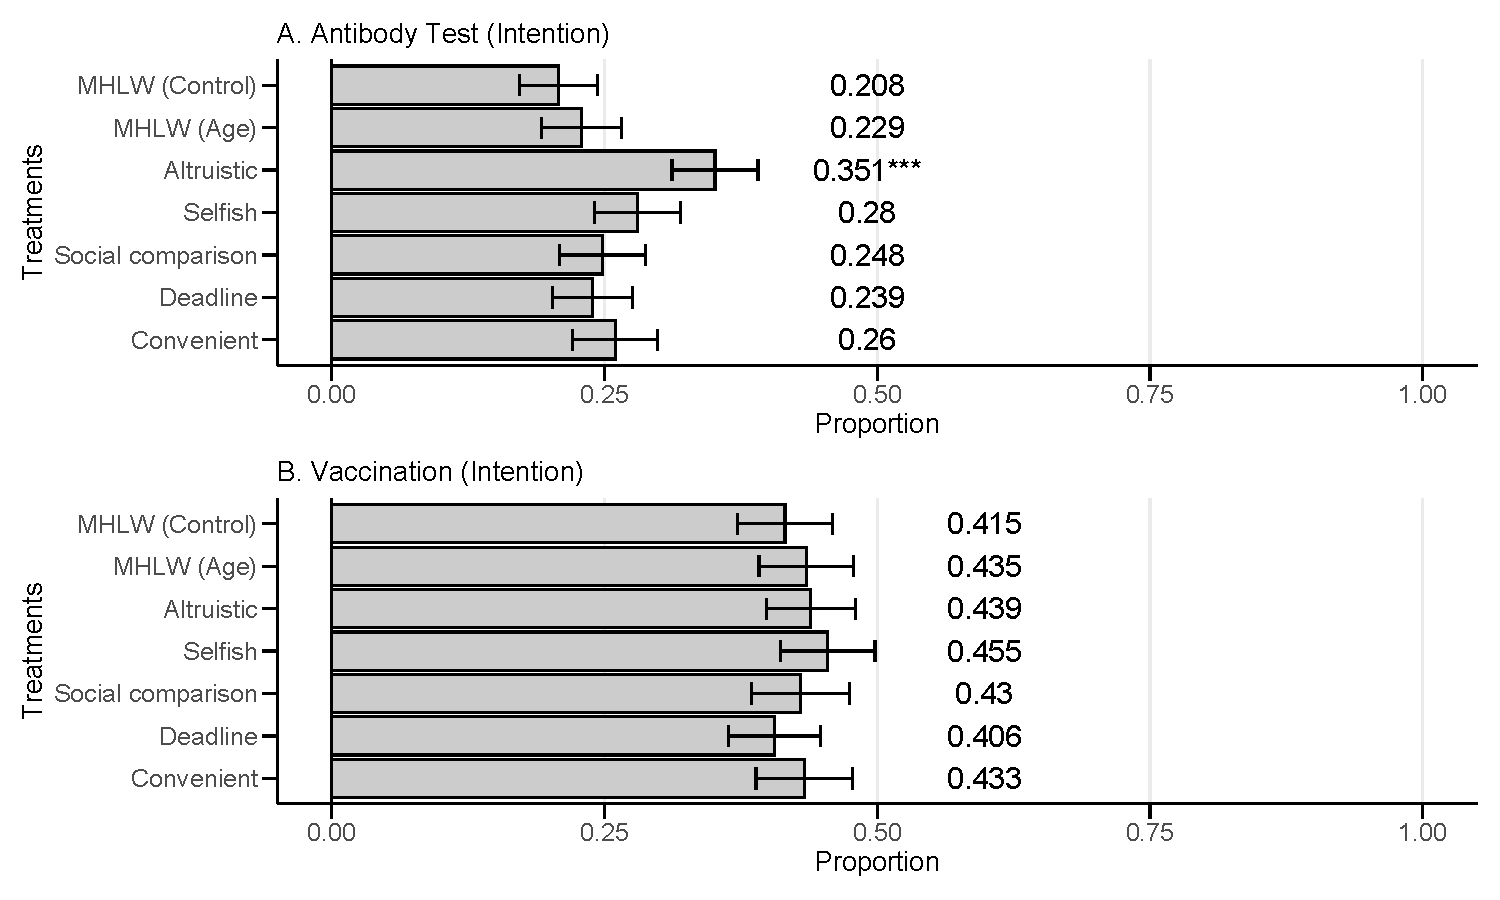
\includegraphics{C:/Users/vge00/Desktop/MHLW-Rubella-Project/2020-online-RCT/publish/body_files/figure-latex/int-coupon1-ttest-1} \caption{Effect of Text-Based Nudges on Intentions among Men for whom Coupons are Automatically Distributed in FY 2019 (N = 927). Data source: wave 1 selection data. Note: Numbers in the figure indicate the proportion of each group. Error bars indicate standard error of the mean. Asterisks are p-values for t-tests of the difference in means from the MHLW message group: * p < 0.1, ** p < 0.05, *** p < 0.01.}\label{fig:int-coupon1-ttest}
\end{figure}

2019年度にクーポン券が自動で送付される男性のサブサンプルを用いて、
我々は各介入群の抗体検査(パネルA)とワクチン接種(パネルB)の意向の比率を
図\ref{fig:int-coupon1-ttest}に示した。
その結果、利他強調メッセージは厚労省メッセージより抗体検査の意向を高めている。
厚労省メッセージ群の抗体検査の意向の比率は約20.8\%であるのに対して、
利他強調メッセージ群の抗体検査の意向の比率は約35.1\%である。
したがって、厚労省メッセージと比較して、
利他強調メッセージは抗体検査の意向を約14.3\%ポイント高めていて、
これは統計的に1\%水準で有意である。

厚労省メッセージと比較して、
すべてのナッジ・メッセージはワクチン接種の意向を統計的に有意に高めていない。
また、すべての介入群のワクチン接種の意向の比率は抗体検査のそれよりも高い。
これはワクチン接種の意向を引き出す質問の刺激によるものだと考えられる。
我々はワクチン接種の意向を回答者に尋ねるとき、抗体を保有していないことを条件にしている。
この条件がワクチン接種の必要性を強く刺激している可能性がある。

\begin{figure}[t]
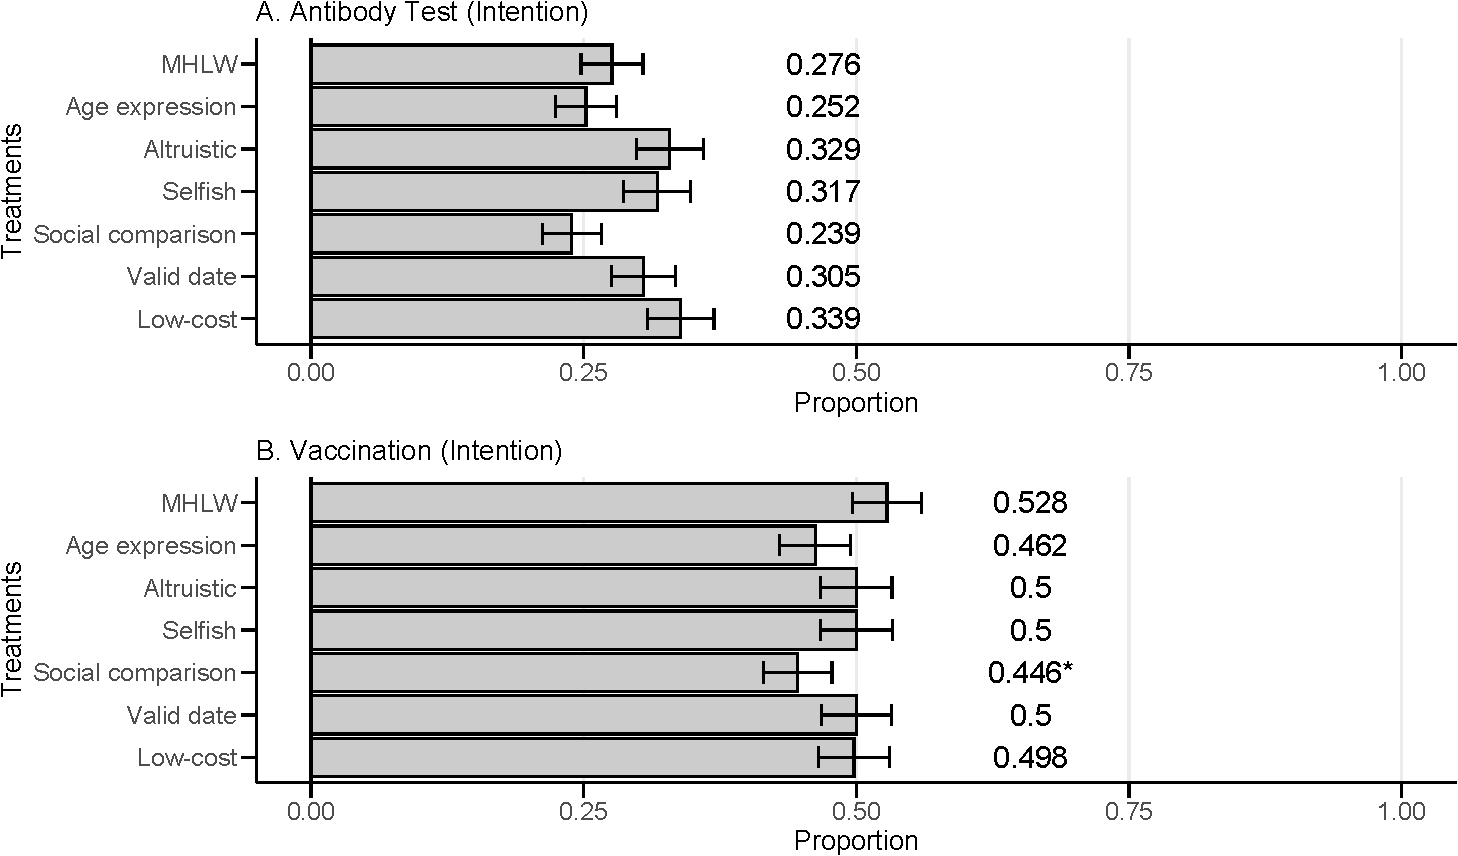
\includegraphics{C:/Users/vge00/Desktop/MHLW-Rubella-Project/2020-online-RCT/publish/body_files/figure-latex/int-coupon0-ttest-1} \caption{Effect of Text-Based Nudges on Intentions among Men Who Needed Costly Procedures to Receive Coupons in FY 2019 (N = 1,688). Data source: wave 1 selection data. Note: Numbers in the figure indicate the proportion of each group. Error bars indicate standard error of the mean. Asterisks are p-values for t-tests of the difference in means from the MHLW message group: * p < 0.1, ** p < 0.05, *** p < 0.01.}\label{fig:int-coupon0-ttest}
\end{figure}

2019年度にクーポン券を得るためにコストのかかる手続きが必要な男性のサブサンプルを用いて、
我々は各介入群の抗体検査(パネルA)とワクチン接種(パネルB)の意向の比率を
図\ref{fig:int-coupon0-ttest}に示した。
その結果、厚労省メッセージと比較して、
すべてのナッジ・メッセージは抗体検査の意向を統計的に有意に高めていない。
対照的に、
社会比較メッセージは厚労省メッセージよりもワクチン接種の意向を低めている。
厚労省メッセージのワクチン接種の意向比率は約52.8\%であるのに対し、
社会比較メッセージのワクチン接種の意向比率は約44.6\%である\footnote{2019年度にクーポン券が自動で送付される男性のサブサンプルを用いた結果と同様に、
  すべての介入群のワクチン接種の意向比率は抗体検査のそれよりも高い。
  これはワクチン接種の意向を引き出す質問の刺激によるものだと考えられる。}。
したがって、厚労省メッセージと比較して、
社会比較メッセージはワクチン接種の意向を約8.2\%ポイント低めており、
これは統計的に10\%水準で有意である。

この効果の原因の一つとして、ワクチン接種のただのりが挙げられる。
社会比較メッセージは「5人に1人が抗体を持っていない」ことを強調している。
裏返せば、5人に4人が抗体を持っているということである。
このメッセージを読んだ人は、
仮に風しんの抗体を保有していないとしても、全体の80\% が抗体を持っているので、
自身が感染する機会は少ないと考えたのかもしれない。
クーポン券を受け取るために手続きが必要なとき、
この信念がワクチンを接種することの価値を低め、
ワクチン接種の意向の比率を厚労省メッセージよりも下げた可能性がある。

クーポン券が自動的に送付されるかどうかは年齢で決まるので、
サブサンプルを用いたナッジ・メッセージの効果は
クーポン券が自動的に送付されるかどうかだけでなく、
二つのサブサンプルの年齢の違いの影響を受けている。
この問題を排除するために、意向の線形確率モデルを推定した。
説明変数はナッジ・メッセージのダミー変数、
ナッジ・メッセージのダミー変数とクーポン券が自動的に送付されることを示すダミー変数の交差項、
そして年齢を含んだ共変量である。
意向の線形確率モデルは上述の結果と同じ結果を得られた(詳細は補論を参照せよ)。

\hypertarget{behavior}{%
\subsection{Effect of Text-Based Nudges on Behaviors}\label{behavior}}

次に、wave 2 selection dataを用いて、
我々は第1回調査以降の行動に対するナッジ・メッセージの効果を推定する。
クーポン券が自動的に送付されるかどうかで分割した2つのサブサンプルにおいて、
個人の観察可能な特徴はトリートメント間でバランスされているので、
t検定の結果のみを示し、回帰分析の結果は補論Cに示す(バランステストの結果は補論Bを見よ)。
また、検定力80\%・有意水準5\%を保つために必要な効果の規模を計算したところ、
2019年度にクーポン券が自動で送付される男性のサブサンプルを用いる場合、少なくとも
7.2
\%ポイントの差が必要である。
2019年度ではクーポン券を受け取るために手続きが必要な男性のサブサンプルを用いる場合、少なくとも
5.3
\%ポイントの差が必要である。

\begin{figure}[t]
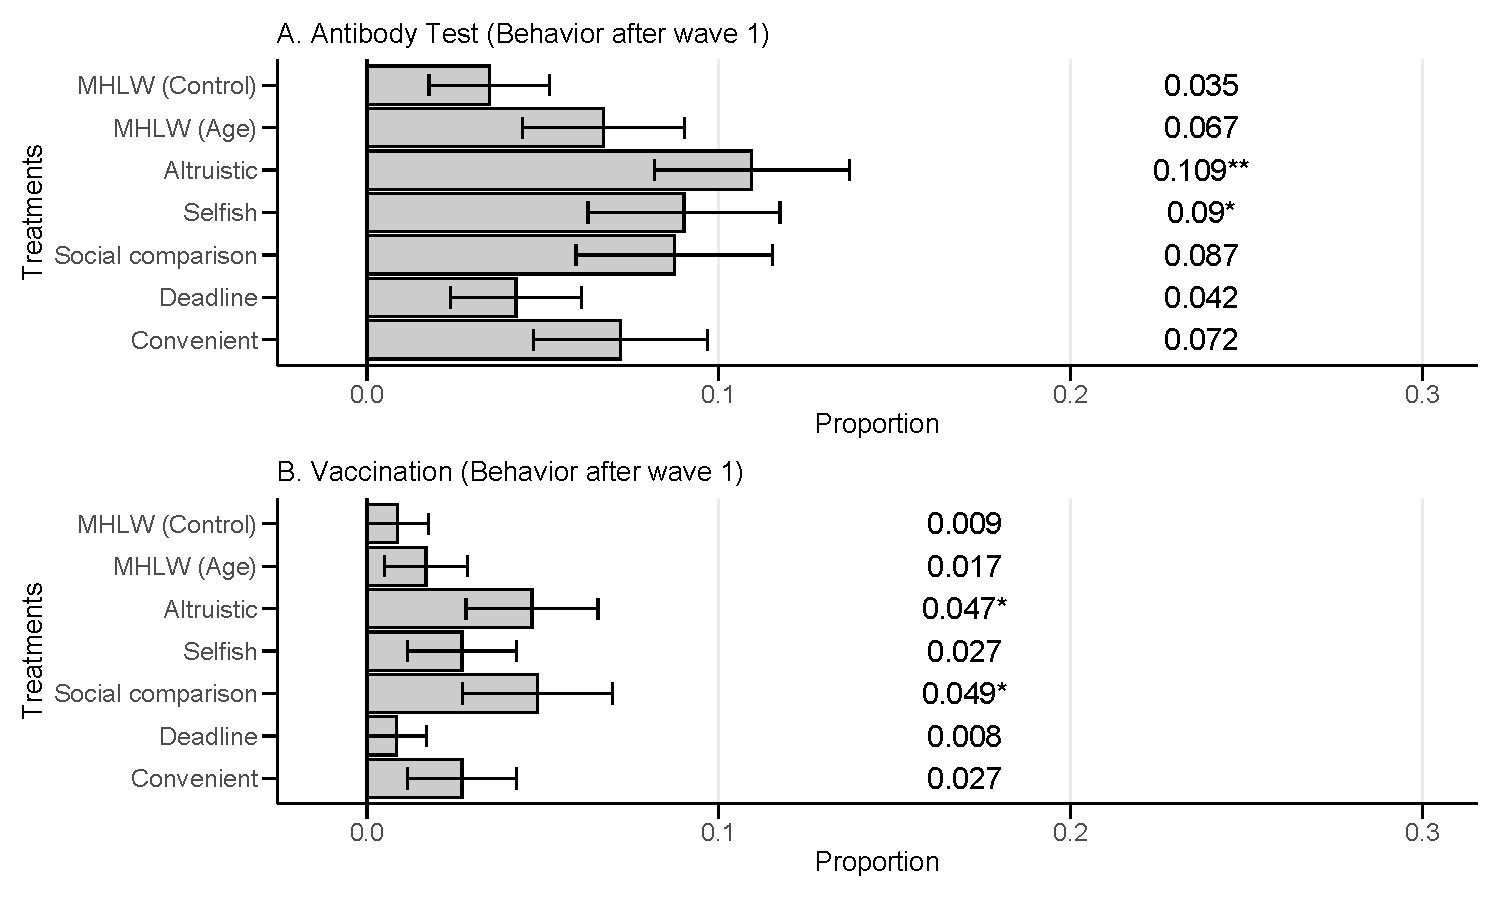
\includegraphics{C:/Users/vge00/Desktop/MHLW-Rubella-Project/2020-online-RCT/publish/body_files/figure-latex/act-coupon1-ttest-1} \caption{Effect of Text-Based Nudges on Behavior among Men for whom Coupons are Automatically Distributed in FY 2019 (N = 805). Data source: wave 2 selection data. Note: Numbers in the figure indicate the proportion of each group. Error bars indicate standard error of the mean. Asterisks are p-values for t-tests of the difference in means from the MHLW message group: * p < 0.1, ** p < 0.05, *** p < 0.01.}\label{fig:act-coupon1-ttest}
\end{figure}

2019年度にクーポン券が自動で送付される男性のサブサンプルを用いて、
我々は各介入群の抗体検査の受検率(パネルA)とワクチン接種率(パネルB)を
図\ref{fig:act-coupon1-ttest}に示した\footnote{ワクチン接種は抗体検査を受検し、ワクチンを接種したら1を取るダミー変数である。
  よって、ワクチン接種率はワクチン接種を通じて新規に抗体を獲得した人の比率とみなすこともできる。
  これは厚生労働省の政策目標と対応するアウトカム変数である。}。
その結果、利他強調メッセージと利己強調メッセージの抗体検査の受検率は厚労省メッセージよりも高い。
厚労省メッセージ群の抗体検査の受検率は約3.5\%である。
対して、利他強調メッセージ群と利己強調メッセージ群の抗体検査の受検率は
それぞれ約10.9\%と約9\%である。
したがって、厚労省メッセージと比較して、
利他強調メッセージは抗体検査の受検率を約7.4\%ポイント引き上げていて、
これは統計的に5\%水準で有意である。
また、利己強調メッセージは抗体検査の受検率を約5.5\%ポイント引き上げており、
これは統計的に10\%水準で有意である。

さらに、利他強調メッセージと社会比較メッセージのワクチン接種率は厚労省メッセージよりも高い。
厚労省メッセージ群のワクチン接種率は約0.9\%である。
対して、利他強調メッセージと社会比較メッセージのワクチン接種率は
それぞれ4.7\%と約4.9\%である。
したがって、厚労省メッセージと比較して、
利他強調メッセージと社会比較メッセージはワクチン接種率を
それぞれ約3.8\%ポイントと4\%ポイント引き上げていて、
これらは統計的に10\%水準で有意である。

\begin{figure}[t]
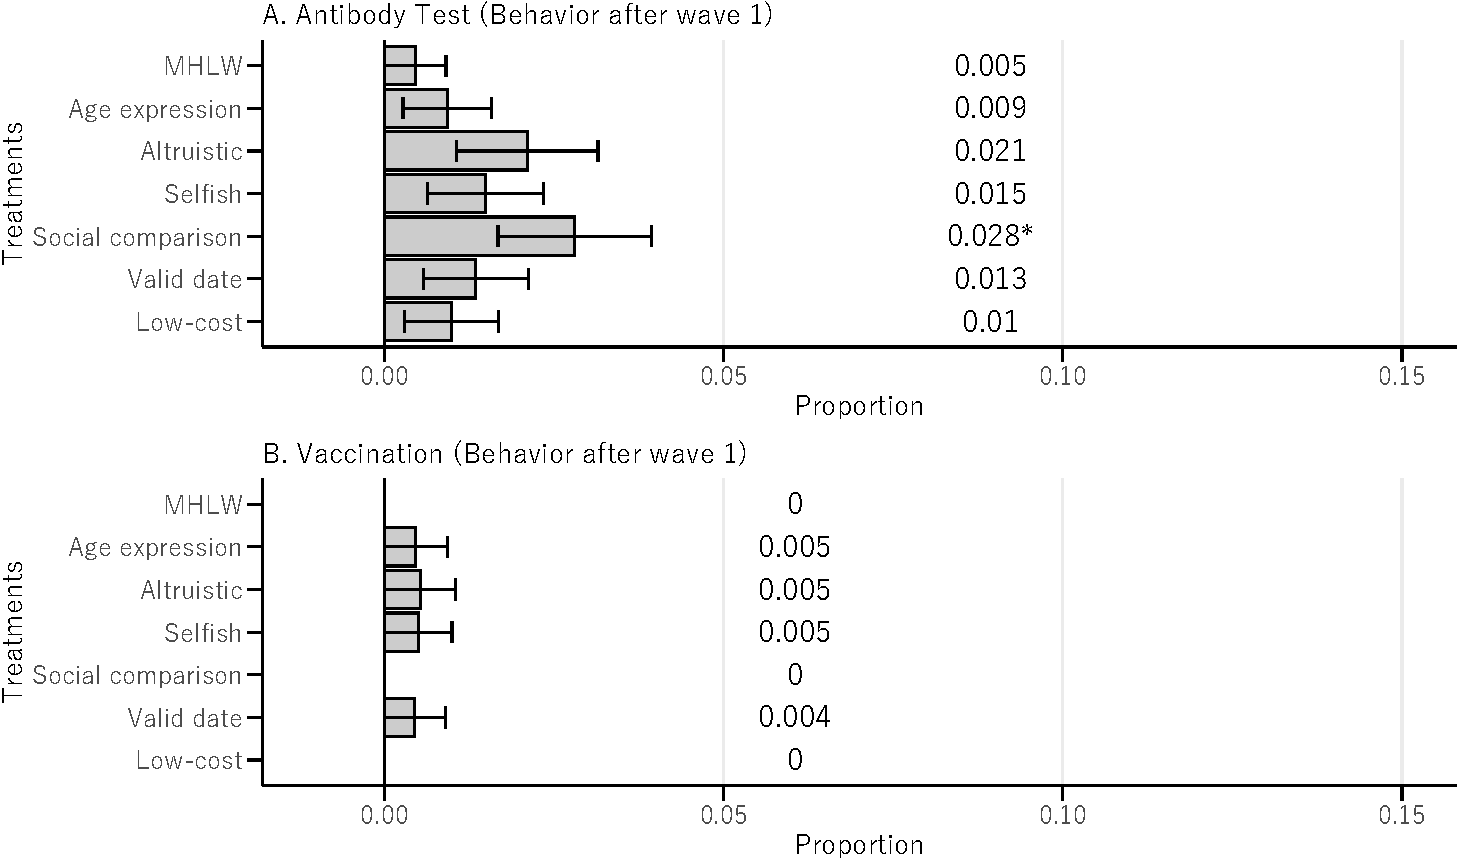
\includegraphics{C:/Users/vge00/Desktop/MHLW-Rubella-Project/2020-online-RCT/publish/body_files/figure-latex/act-coupon0-ttest-1} \caption{Effect of Text-Based Nudges on Behaviors among Men Who Needed Costly Procedures to Receive Coupons in FY 2019 (N = 1,467). Data source: wave 1 selection data. Note: Numbers in the figure indicate the proportion of each group. Error bars indicate standard error of the mean. Asterisks are p-values for t-tests of the difference in means from the MHLW message group: * p < 0.1, ** p < 0.05, *** p < 0.01.}\label{fig:act-coupon0-ttest}
\end{figure}

2019年度にクーポン券を得るためにコストのかかる手続きが必要な男性のサブサンプルを用いて、
我々は各介入群の抗体検査の受検率(パネルA)とワクチン接種率(パネルB)を
図\ref{fig:act-coupon0-ttest}に示した。
その結果、厚労省メッセージと比較して、
社会比較メッセージは抗体検査の受検率を高めているが、
ワクチン接種率を高めていない。
厚労省メッセージを読んだ人の0.5\%が抗体検査を受検しているが、
誰もワクチン接種をしていない。
同様に、社会比較メッセージを読んだ人の2.8\%が抗体検査を受検しているが、
誰もワクチン接種をしていない。
したがって、厚労省メッセージと比較して、
社会比較メッセージは抗体検査の受検率を約2.3\%ポイント引き上げていて、
これは統計的に10\%水準で有意である。
しかしながら、ワクチン接種率に対する効果はゼロである。

サブサンプルで推定されたナッジ・メッセージの効果は
クーポン券が自動的に送付されるかどうかだけでなく、
年齢の違いの影響を受けるので、
我々はこの問題を排除するために線形確率モデルを推定した。
行動の線形確率モデルは上述の結果と同じ結果を得られた。
それに加えて、2019年度にクーポン券が自動的に送付される男性において、
社会比較メッセージの抗体検査の受検率は厚労省メッセージよりも5.7\%ポイント高く、
これは統計的に10\%水準で有意である。

\begin{table}

\begin{threeparttable}
\caption{\label{tab:tester-move}Movement of Antibody Test Takers}
\centering
\fontsize{9}{11}\selectfont
\begin{tabular}[t]{>{\raggedright\arraybackslash}p{9em}>{\centering\arraybackslash}p{5em}>{\centering\arraybackslash}p{5em}>{\centering\arraybackslash}p{5em}>{\centering\arraybackslash}p{5em}>{\centering\arraybackslash}p{5em}>{\centering\arraybackslash}p{5em}}
\toprule
\multicolumn{1}{c}{ } & \multicolumn{3}{c}{w/ receiving coupon automatically} & \multicolumn{3}{c}{w/o receiving coupon automatically} \\
\cmidrule(l{3pt}r{3pt}){2-4} \cmidrule(l{3pt}r{3pt}){5-7}
Text-based nudge & Antibody test & Negative test result & Vaccination & Antibody test  & Negative test result  & Vaccination \\
\midrule
MHLW (Control) & 4 & 1 & 1 & 1 & 0 & 0\\
MHLW (Age) & 8 & 2 & 2 & 2 & 2 & 1\\
Altruistic & 14 & 7 & 6 & 4 & 1 & 1\\
Selfish & 10 & 3 & 3 & 3 & 1 & 1\\
Social comparison & 9 & 5 & 5 & 6 & 1 & 0\\
Deadline & 5 & 1 & 1 & 3 & 1 & 1\\
Convenient & 8 & 5 & 3 & 2 & 0 & 0\\
Fisher's exact test (p-value) &  & 0.55 & 0.67 &  & 0.47 & 1.00\\
\bottomrule
\end{tabular}
\begin{tablenotes}
\small
\item [] Note: Limiting our sample to antibody test takers, we tested the null hypothesis that the number of negative antibody tests does not differ between intervention groups with Fisher's exact test. Also, restricting the sample to negative individuals, we tested the null hypothesis that the number of vaccinations would not differ between intervention groups with a Fisher's exact test.
\end{tablenotes}
\end{threeparttable}
\end{table}

クーポン券が自動的に送付されるかどうかに関わらず、
すべての群において、ワクチン接種率は抗体検査の受験率より低い。
これは陰性であるにも関わらずワクチンを接種していない人が多いからではなく、
ワクチンを接種するべき人が少ないという外生的な要因によるものである。
この点を明らかにするために、
我々は抗体検査の受検者数・抗体検査が陰性であった人の数・ワクチンを接種した人数を
介入群ごとに計算し、表\ref{tab:tester-move}に示した。

表\ref{tab:tester-move}より、
クーポン券が自動的に送付されかどうかや介入群に関わらず
抗体検査の結果が陰性である人のほとんどがワクチンを接種している\footnote{2019年度にクーポン券を自動的に受け取った男性に限定すると、
  陰性者のワクチン接種率は87.5\%(\(=21/24\))であり、
  1000個のブートストラップ標本を用いて構築した95\%信頼区間は
  {[}75.0\%, 100.0\%{]}
  である。
  2019年度にクーポン券を受け取るためにはコストのかかる手続きが必要な男性に限定すると、
  陰性者のワクチン接種率は66.7\%(\(=4/6\))であり、
  1000個のブートストラップ標本を用いて構築した95\%信頼区間は
  {[}33.3\%, 100.0\%{]}
  である。}。
2019年度にクーポン券を自動的に受け取った男性に限定すると、
利他強調メッセージ・低コストメッセージを除くすべての群で
陰性者はワクチンを接種している。
また、利他強調メッセージ・低コストメッセージ群においても
ワクチンを接種していない陰性者は少数である。
同様に、2019年度にクーポン券を受け取るためにはコストのかかる手続きが必要な男性に限定すると、
年齢表現メッセージ・社会比較メッセージを除くすべての群で
陰性者はワクチンを接種している。

さらに、表\ref{tab:tester-move}より、
抗体検査の陰性件数が介入群間でバラツキがあることが分かる。
2019年度にクーポン券を自動的に受け取った男性に限定したとき、
厚労省メッセージの抗体検査の陰性比率は25\%(\(=1/4\))である。
これに対して、ワクチン接種率に対して効果のある
利他強調メッセージ・社会比較メッセージの抗体検査の陰性比率は
それぞれ50\%(\(=7/14\))・55\%(\(=5/9\))である。
逆に、抗体検査受検率のみに効果のある利己強調メッセージの抗体検査の陰性比率は
30\%(\(=3/10\))であり、
厚労省メッセージのそれと近い値を取る。
2019年度にクーポン券を受け取るためにはコストのかかる手続きが必要な男性に限定するとき、
抗体検査受検率のみに効果のある社会比較メッセージの抗体検査の陰性比率は16\%(\(=1/6\))である。
したがって、
ワクチン接種率が高い介入群は陰性比率が高く、
それがワクチン接種率に対する効果に影響を与えたといえる。

ただし、抗体検査の陰性比率の介入群間のばらつきは統計的な誤差による可能性が高い。
我々はクーポン券を自動的に送付される対象かどうかでサンプルを分割し、
抗体検査の陰性件数が介入群間で異ならないという帰無仮説を
フィッシャーの正確検定で検証した。
その結果、二つのサブサンプルでこの帰無仮説を棄却できない。
よって、我々のデータの抗体検査の陰性比率は介入群間で異なっているが、
母集団のそれは介入群間で異ならないかもしれない\footnote{これと対立する仮説として、
  利他強調メッセージや社会比較メッセージを読んで抗体検査を受検した人は
  自身に抗体を保有していないと信じているということが考えられる。
  そこで、陰性者の抗体検査受検率を推定することを試みる。
  しかしながら、陰性であるにも関わらず抗体検査を受検していない人がいるはずなので、
  陰性者の抗体検査受検率をデータから直接復元することはできない。
  ベイズ定理を用いて、我々は間接的に推定した。
  陰性という事象\(A\)と抗体検査の受検という事象\(B\)の二つの事象を考える。
  このとき、抗体検査の受検比率は\(P(B)\)、抗体検査受検者の陰性比率は\(P(A|B)\)で表すことができ、
  これらの値はデータから直接推定できる。
  ベイズの定理より、抗体検査受検者の陰性比率は
  \[ P(A|B) = \frac{P(B|A) \cdot P(A)}{P(B)} \]
  と定義できる。
  ここで、\(P(A)\)は陰性比率であり、
  これはNIIDの抗体保有率のデータより0.2となる。
  確率\(P(B|A)\)は陰性者で条件づけた抗体検査の受検比率であり、我々の関心のあるパラメータである。
  よって、陰性者の抗体検査の受検比率は
  \[ \hat{P}(B|A) = \frac{\hat{P}(A|B) \cdot \hat{P}(B)}{0.2} \]
  で計算できる。
  利他強調メッセージ群において、
  \(\hat{P}(A|B) = 0.5\)と\(\hat{P}(B) = 0.109\)なので、
  \(\hat{P}(B|A) = 0.273\)となる(1000個のブートストラップ標本で構築した95\%信頼区間は
  {[}0.117, 0.469{]}
  さらに、陰性であるかどうかによって抗体検査の受検にセレクションが生じているかどうかを
  検証するために、陰性という事象と抗体検査の受検という事象が独立であるという帰無仮説を検定した。
  \(\hat{P}(B|A) - \hat{P}(B)\)の95\%信頼区間にゼロが含まれていないとき、
  我々は帰無仮説を5\%有意水準で棄却できる。
  その結果、\(\hat{P}(B|A) - \hat{P}(B)\)の95\%信頼区間は
  {[}0.016, 0.336{]}
  なので、我々は帰無仮説を棄却できる。
  同様に、社会比較メッセージ群の\(\hat{P}(B|A) - \hat{P}(B)\)の95\%信頼区間は
  {[}0.000, 0.350{]}
  である。
  したがって、利他強調メッセージ群と社会比較メッセージ群では、
  陰性者が抗体検査を積極的に受検している傾向があるかもしれない。}。

\hypertarget{econvalue}{%
\subsection{Monetary Value of Text-Based Nudges}\label{econvalue}}

厚生労働省の追加施策は風しんワクチンの価格をゼロにする金銭的インセンティブとみなせる。
しかしながら、クーポン券を利用した抗体検査の受検率は18\%である。
抗体検査の結果が陰性であれば、ワクチン接種を受ける必要がないので、
クーポン券を利用したワクチン接種率は18\%より低くなる。
では、仮に、厚生労働省がナッジ・メッセージを用いずに金銭的インセンティブだけを用いて、
ワクチン接種率を高めようとしているならば、
厚生労働省はあといくらの追加的な金銭的インセンティブを個人に与えればよいのだろうか。

そこで、我々はオンライン調査で得られた風しんワクチン接種の支払意思額を用いて、
ナッジ・メッセージの効果を金銭的な価値を評価する。
ナッジ・メッセージの効果の金銭的な価値は
推定されたメッセージの効果と同等となる追加的な金銭的補助である。
似たようなアプローチでナッジ・メッセージの金銭的な価値を推定した研究に
Bursztyn et al. (2019) や Moriwaki et al. (2020) がある。

我々は、第1回調査のナッジ・メッセージを示す前に、ワクチン接種の支払意思額を調査した。
ワクチンの価格は5000円と仮定して、
我々は、自治体の補助金額が\(s_j\)のとき、ワクチン接種をするかどうかを調査した。
補助金額は\(s_j \in \{0, 1000, 2000, \ldots, 10000\}\)とした。
回答者\(i\)が接種すると回答した最低の補助金額を\(s_i^{\text{min}}\)とする。
回答者\(i\)が接種しないと回答した最高の補助金額を\(s_i^{\text{max}}\)とする。
このとき、回答者\(i\)の支払意思額は
\([5000 - s_i^{\text{min}}, 5000 - s_i^{\text{max}})\)の範囲内で識別される\footnote{回答者がすべての補助金額\(s_j\)のときの接種しないと回答したならば、\(s_i^{\text{max}} = 10000\)である。
  しかしながら、\(s_i^{\text{min}}\)はデータで定義できない。そこで、\(s_i^{\text{min}} = 11000\)と仮定した。
  ただし、後に示すが、この仮定はナッジ・メッセージの金銭的価値に影響を与えない。}。
したがって、
追加の仮定を置かない限り、ワクチン接種の需要曲線はステップワイズな曲線となり、
メッセージの金銭的価値は範囲で得られる。

メッセージの金銭的価値を点推定するために、
我々は支払意思額が
\([5000 - s_i^{\text{min}}, 5000 - s_i^{\text{max}})\)の範囲で
識別されるとき、
真の支払意思額はその範囲内で一様に分布することを仮定する。
このとき、ステップワイズなワクチン接種の需要曲線は線型補間で表される。
我々は補論に支払意思額に関する調査と需要曲線を示した。

\begin{table}

\caption{\label{tab:economic-value}Estimated Monetary Value of Text-Based Nudges}
\centering
\resizebox{\linewidth}{!}{
\fontsize{9}{11}\selectfont
\begin{threeparttable}
\begin{tabular}[t]{lcccccc}
\toprule
\multicolumn{3}{c}{ } & \multicolumn{2}{c}{Monetary value (JPY)} & \multicolumn{2}{c}{Monetary value (USD)} \\
\cmidrule(l{3pt}r{3pt}){4-5} \cmidrule(l{3pt}r{3pt}){6-7}
Text-based nudge & Size of effect & Baseline + size of effect & pp & total & pp  & total \\
\midrule
MHLW (Age) & 0.032 & 0.732 & 367.854 & 1.946 & 3.344 & 17.690\\
Altruistic & 0.075 & 0.774 & 2037.553 & 10.779 & 18.523 & 97.988\\
Selfish & 0.055 & 0.755 & 744.045 & 3.936 & 6.764 & 35.782\\
Social comparison & 0.053 & 0.752 & 596.335 & 3.155 & 5.421 & 28.678\\
Deadline & 0.008 & 0.707 & 86.059 & 0.455 & 0.782 & 4.139\\
Convenient & 0.037 & 0.737 & 422.789 & 2.237 & 3.844 & 20.332\\
\bottomrule
\end{tabular}
\begin{tablenotes}
\item Note: Effect is the size of effect of each text-based nudge on antibody test. Baseline is the sum of the rate of antibody test in the control and the vaccination rate when the vaccine is free The monetary value is the amount per person (pp) and the total amount (total) multiplied by the number of people who received the coupon in 2019 but did not use it until January, 2020. We valued the monetary value in Japanese Yen (JPY) and US Dollars (USD) (1USD = 110JPY). The unit of monetary value per person is 1 JPY and 1 USD, respectively. The unit of total monetary value is 1 billion JPY and 1 million USD, respectively.
\end{tablenotes}
\end{threeparttable}}
\end{table}

ナッジ・メッセージの金銭的な価値を次のように計算する。
はじめに、ベースラインの接種割合を決める。
クーポン券が自動的に配布され、抗体検査やワクチン接種を受検していない人に限定して、
需要曲線を推定した。
したがって、ワクチンの供給曲線はゼロで水平である。
このときの接種割合は約66.5\%である。
ベースラインの接種割合はこの割合に
厚労省メッセージの抗体検査受検率を足したものである\footnote{ベースラインの接種割合を求めるときに、
  我々は厚労省メッセージの抗体検査受検率を足した。
  これは調査によってメッセージを受け取ることの自体の影響を考慮したためである。}。
ベースラインの接種割合は約70\%であり、対応する支払意思額は約-394円である。

次に、
接種割合をベースラインの均衡点からナッジ・メッセージの効果分だけ増やすとき、
需要曲線上で対応する支払意思額を見つける。
その支払意思額は
ナッジ・メッセージの効果だけ増やすのに必要な自治体の追加的な補助金額であり、
それがナッジ・メッセージの一人当たりの金銭的価値である。
たとえば、
ベースラインの均衡点の接種割合とナッジ・メッセージの効果の和が0.8であるとき、
需要曲線上で対応する支払意思額は約-4280円である。
すなわち、ナッジ・メッセージの効果量分だけ接種割合を増やすために、
自治体は一人当たり約3886(\(=4280-394\))円の追加的な補助金を支払う必要がある。

我々は抗体検査の受検率に対するナッジ・メッセージの効果を用いる。
表\ref{tab:tester-move}で示したように、
抗体検査の結果が陰性である人のほとんどはワクチンを接種している。
この事実は、抗体検査を受検した人は同時にワクチンを接種したいと考えている
ことを示唆している。
したがって、抗体検査受検に対するナッジ・メッセージの効果を
行動から推測されるワクチン接種の(真の)意向に対する効果とみなせる。

表\ref{tab:economic-value}はメッセージの金銭的価値の試算結果である。
第2列は図\ref{fig:act-coupon1-ttest}の
パネルAで示したメッセージの効果を示している。
第3列はベースラインの均衡点の接種割合から
メッセージの効果だけ増やしたときの接種割合を示している。
第4列はメッセージの一人当たりの金銭的価値である。
この金銭的価値をアメリカドルに換算した結果を第6列に示している。
抗体検査の受検を促進した利他強調メッセージの一人当たりの金銭的価値は約2000円(約18ドル)である。

また、メッセージ自体の金銭的価値の総額は一人当たりの金銭的価値と
2019年度に発行されたクーポン券をまだ利用していない人数の積で得られる。
厚生労働省より、2019年度にクーポン券が発行されたにもかかわらず、
1月時点で抗体検査のクーポン券を利用していない人は約529万人である。
表\ref{tab:economic-value}の第5列はメッセージの金銭的価値の総額を示している。
第7列はそれをアメリカドルに換算した結果を示している。
利他強調メッセージの金銭的価値の総額は約100億円である。

\hypertarget{conclusion}{%
\section{Discussion and Conclusions}\label{conclusion}}

本研究は、オンラインサーベイによるランダム化比較試験(RCT)を用いて、
風しんワクチンの接種を促進するためにどのようなナッジ・メッセージが有効であるかを明らかにした。
主な結果は以下の三つにまとめられる。
第一に、2019年度にクーポン券送付対象の年齢の男性のみに
利他強調メッセージが抗体検査の受検を7.5\%ポイント促進した。
この効果は個人の観察可能な特徴に対して頑健である。
このメッセージの効果を金銭的価値で評価すると、
一人当たりの金銭的価値は約2000円(約18ドル)であり、
その総額は約100億円(約9,700万ドル)である。

利己強調メッセージや社会比較メッセージも抗体検査を促進している可能性がある。
二群の平均値の差の検定より、
利己強調メッセージは統計的な有意性は弱いものの、抗体検査を促進していた。
共変量を制御した線形確率モデルより、
利己強調メッセージや社会比較メッセージは統計的な有意性は弱いが、
抗体検査を促進していた。
さらに、線形確率モデルの推定値を用いて、
利他強調メッセージを参照群としたメッセージの効果を推定した。
その結果、利己強調メッセージや社会比較メッセージの抗体検査の受検比率は
利他強調メッセージ群のそれと有意な差ではない。
この意味で、二つのメッセージも抗体検査の受検を促進した可能性がある。
しかしながら、
抗体検査の受検比率の差は検出力を十分に保てるほどの大きさではないので、
サンプルサイズを増やした再検証が必要である。

第二に、クーポン券を自動的に受け取ったかどうか・介入群に関わらず、
抗体検査の結果が陰性である人のほとんどはワクチンを接種していた。
よって、
ワクチン接種率に対するメッセージの効果は介入群の陰性比率に強く依存している。
これは陰性比率を高めるようなナッジ・メッセージがワクチン接種率を高めることを
示唆している。
本研究で用いたナッジ・メッセージが陰性比率を高めているようなエビデンスは
得られなかった。これは抗体検査の受験者数が少なすぎる可能性も考えられる。
自治体の接種データなどでの大規模なデータを活用した再検証が必要である。

この結果はナッジ・メッセージのターゲティングに関する問題も提供している。
すなわち、全員がワクチン接種を促進するようなナッジ・メッセージか、
もしくは感染しやすい人を促進するようなナッジ・メッセージのどちらが
社会的に効率的なのかという問題である。
これは日本の風しん政策だけでなく、一般的なワクチン政策に適用される問題だろう。

最後に、
2019年度にクーポン券を受け取るためにはコストのかかる手続きが必要な男性に対して、
ナッジ・メッセージの効果は弱い。
考えられる可能性が二つある。
第一に、厚生労働省の無料クーポン券制度を認知度が低い点である。
第1回調査の調査票A(ナッジ・メッセージを示す前の調査)で、
我々は厚生労働省のクーポン券制度の認知度を調査した。
その結果、クーポン券を受け取るのに手続きが必要な男性の約77.5\%
が厚生労働省のクーポン券制度を知らなかった。
仮にナッジ・メッセージを読んで、
風しんの抗体検査やワクチン接種を受ける必要性を理解したとしても、
クーポン券の存在を知らない人は
それらの予防行動を自費で受けないといけないと考えている。
ナッジ・メッセージは
予防行動のコストを上回るほどその価値を高められなかったのかもしれない。
第二に、クーポン券制度を認知し、無料で受けられることを知っていたとしても、
自治体にクーポン券を発行してもらうように依頼する必要があるという点である。
クーポン券制度を認知している男性が
無料で抗体検査やワクチン接種を受けられることを知っていても、
クーポン券の発行の手続き自体にコストが伴う。
したがって、ナッジ・メッセージはクーポン券の発行の手続きのコストを上回るほどその価値を高められなかったのかもしれない。

本研究の限界として、行動に関するアウトカムがすべて自己申告によるものである。
アウトカム変数に想起バイアスや虚偽の回答が含まれているならば、
推定された効果は真の効果ではない。

本研究では、抗体検査やワクチン接種の有無について誤報告はないと仮定して、分析をした。
接種時期が近ければ近いほど、この仮定は妥当性を帯びてくると考えている。
したがって、第1回調査以降に抗体検査やワクチン接種を受けたかどうかの回答はある程度信頼できる。
また、第1回調査で抗体検査もしくはワクチン接種を受けたと回答した人を除いたデータを用いて、
我々は時期に基づかない行動に関するアウトカム変数に対する効果を推定した。
その結果、
効果・統計的な有意性・効果の金銭的価値は大きく異なるものの、
利他強調メッセージが2019年度にクーポン券が自動的に送付された人の抗体検査の受検を
促進していることを確認している(詳細は補論を参照せよ)。

自己申告に関する問題点を完全に回避するためには、
行政データなどの客観的な指標を用いる必要がある。
これは将来の課題である。

\newpage

\hypertarget{references}{%
\section*{References}\label{references}}
\addcontentsline{toc}{section}{References}

\hypertarget{refs}{}
\begin{CSLReferences}{1}{0}
\leavevmode\vadjust pre{\hypertarget{ref-Bursztyn2019}{}}%
Bursztyn, L., Fiorin, S., Gottlieb, D., Kanz, M., 2019. Moral {Incentives} in {Credit Card Debt Repayment}: {Evidence} from a {Field Experiment}. Journal of Political Economy 127, 1641--1683. doi:\href{https://doi.org/10.1086/701605}{10.1086/701605}

\leavevmode\vadjust pre{\hypertarget{ref-Dai2021}{}}%
Dai, H., Saccardo, S., Han, M.A., Roh, L., Raja, N., Vangala, S., Modi, H., Pandya, S., Sloyan, M., Croymans, D.M., 2021. Behavioural nudges increase {COVID-19} vaccinations. Nature 597, 404--409. doi:\href{https://doi.org/10.1038/s41586-021-03843-2}{10.1038/s41586-021-03843-2}

\leavevmode\vadjust pre{\hypertarget{ref-Kinoshita2016}{}}%
Kinoshita, R., Nishiura, H., 2016. Assessing herd immunity against rubella in {Japan}: A retrospective seroepidemiological analysis of age-dependent transmission dynamics. BMJ Open 6, e009928. doi:\href{https://doi.org/10.1136/bmjopen-2015-009928}{10.1136/bmjopen-2015-009928}

\leavevmode\vadjust pre{\hypertarget{ref-Milkman2021}{}}%
Milkman, K.L., Patel, M.S., Gandhi, L., Graci, H.N., Gromet, D.M., Ho, H., Kay, J.S., Lee, T.W., Akinola, M., Beshears, J., Bogard, J.E., Buttenheim, A., Chabris, C.F., Chapman, G.B., Choi, J.J., Dai, H., Fox, C.R., Goren, A., Hilchey, M.D., Hmurovic, J., John, L.K., Karlan, D., Kim, M., Laibson, D., Lamberton, C., Madrian, B.C., Meyer, M.N., Modanu, M., Nam, J., Rogers, T., Rondina, R., Saccardo, S., Shermohammed, M., Soman, D., Sparks, J., Warren, C., Weber, M., Berman, R., Evans, C.N., Snider, C.K., Tsukayama, E., Van den Bulte, C., Volpp, K.G., Duckworth, A.L., 2021. A megastudy of text-based nudges encouraging patients to get vaccinated at an upcoming doctor's appointment. Proc Natl Acad Sci USA 118, e2101165118. doi:\href{https://doi.org/10.1073/pnas.2101165118}{10.1073/pnas.2101165118}

\leavevmode\vadjust pre{\hypertarget{ref-Moriwaki2020}{}}%
Moriwaki, D., Harada, S., Schneider, J., Hoshino, T., 2020. Nudging Preventive Behaviors in COVID-19 Crisis: A Large Scale RCT using Smartphone Advertising (No. DP2020-021), Keio-IES Discussion Paper Series. {Institute for Economic Studies, Keio University}, {Tokyo, Japan}.

\end{CSLReferences}

\end{document}
